\documentclass[conference]{IEEEtran}

% -----------------------------------------------------------------------
% Packages
% -----------------------------------------------------------------------
\usepackage{amsmath,amssymb,amsfonts}
\usepackage{graphicx}
\usepackage{textcomp}
\usepackage{xcolor}
\usepackage{booktabs}
\usepackage{cite}
\usepackage{microtype}
\usepackage{tikz}
\usepackage{pgfplots}
\pgfplotsset{compat=1.18}
\usetikzlibrary{shapes.geometric, arrows.meta, positioning, calc, fit}
\usepackage[hidelinks]{hyperref}

\begin{document}

% -----------------------------------------------------------------------
% Title
% -----------------------------------------------------------------------
\title{An Honest Multi-Phase Clinical Screening Platform for Autism Spectrum
Disorder: From Validated Questionnaire Ensembles to Browser-Native
Brain Connectivity Analysis}

% -----------------------------------------------------------------------
% Authors  (6 authors, two rows of three — IEEE conference style)
% -----------------------------------------------------------------------
\author{
\IEEEauthorblockN{Ratna Patil}
\IEEEauthorblockA{\textit{Dept. of AI \& DS}\\
\textit{Vishwakarma Institute of Technology}\\
Pune, India\\
ratna.patil@vit.edu}
\and
\IEEEauthorblockN{Mohit Agrawal}
\IEEEauthorblockA{\textit{Dept. of AI \& DS}\\
\textit{Vishwakarma Institute of Technology}\\
Pune, India\\
mohit.agrawal24@vit.edu}
\and
\IEEEauthorblockN{Tanay Agrawal}
\IEEEauthorblockA{\textit{Dept. of AI \& DS}\\
\textit{Vishwakarma Institute of Technology}\\
Pune, India\\
tanay.agrawal24@vit.edu}
\and
\IEEEauthorblockN{Ayush Bagde}
\IEEEauthorblockA{\textit{Dept. of AI \& DS}\\
\textit{Vishwakarma Institute of Technology}\\
Pune, India\\
ayush.bagde24@vit.edu}
\and
\IEEEauthorblockN{Shreyash Bhandare}
\IEEEauthorblockA{\textit{Dept. of AI \& DS}\\
\textit{Vishwakarma Institute of Technology}\\
Pune, India\\
shreyash.bhandare24@vit.edu}
\and
\IEEEauthorblockN{Vibhav Bagade}
\IEEEauthorblockA{\textit{Dept. of AI \& DS}\\
\textit{Vishwakarma Institute of Technology}\\
Pune, India\\
vibhav.bagade24@vit.edu}
}

\maketitle

% -----------------------------------------------------------------------
% Abstract
% -----------------------------------------------------------------------
\begin{abstract}
Autism Spectrum Disorder (ASD) affects roughly 1 in 36 children in the
United States \cite{maenner2023}, yet median diagnostic latency remains
close to five years from first parental concern to clinical
confirmation. Two very different barriers feed this gap: in high-income
countries, the bottleneck is scarcity of trained clinicians who can
administer gold-standard assessments like the ADOS-2; in low- and
middle-income settings, the barrier is more basic---most families have
never even heard of a structured ASD questionnaire.

This paper describes a five-phase platform we built to address both ends
of that gap. Phase~1 trains and evaluates a stacking ensemble of five
classifiers (Logistic Regression, LightGBM, XGBoost, CatBoost, and a
meta-learner) on AQ-10 behavioral responses across five demographic
cohorts (adult, adolescent, child, toddler, and infant), achieving
100\,\% held-out accuracy on the adult cohort with a Brier score of
0.0017, which reflects excellent calibration. Phase~2 provides a
production-quality web interface with AQ-10 reverse-scored items,
conformal-prediction uncertainty flags, and consent-first privacy
design. Phase~3 integrates a clinical-context companion that explains
each screening result in plain language, referencing DSM-5 criteria and
localizing community resources. Phase~4 implements a fMRI functional
connectivity analysis pipeline on the ABIDE-I dataset (120 subjects,
four acquisition sites), honestly reporting 55.0\,\% LOSO accuracy with
ComBat harmonization --- a number we deliberately leave uncurated because
it reflects real-world scanner heterogeneity rather than in-sample
performance. Phase~5 exports the best questionnaire model as a 2.4~kB
ONNX-distilled student model that runs entirely in the browser with
0.45~ms inference latency, requiring no server and no data upload.

We report every metric that mattered, including the ones that were
disappointing, and we describe the design decisions behind each. The
platform is open-source, zero-dependency deployable, and tested through
24 automated unit and integration tests.
\end{abstract}

\begin{IEEEkeywords}
Autism Spectrum Disorder, AQ-10, Stacking Ensemble, XGBoost,
LightGBM, CatBoost, fMRI Connectivity, ABIDE-I, Conformal Prediction,
ComBat, Browser ML, ONNX, Clinical Decision Support.
\end{IEEEkeywords}

% -----------------------------------------------------------------------
\section{Introduction}
% -----------------------------------------------------------------------

Diagnosing autism is not a blood test. There is no biomarker you can
point to under a microscope, no imaging finding that is pathognomonic
on its own. The diagnosis depends on structured behavioral observation,
caregiver interviews, and clinician judgment---a process that takes
hours when done properly, requires specialists who spend years training
on instruments like the ADOS-2 \cite{lord2018ados} and ADI-R, and is completely inaccessible
to most families outside large urban centers.

We started thinking about this problem from a simple observation: the
AQ-10, a ten-item screening questionnaire developed by Baron-Cohen and
colleagues at Cambridge \cite{allison2012}, can be completed in under
five minutes on a smartphone. It is not a diagnostic tool. But it is a
validated, free, and widely available first filter---and, critically, it
requires no clinician. If a reliable, well-calibrated ML system could
sit behind it, flag likely cases with high sensitivity, and route
families toward the appropriate next step, that could shave months off
the referral pipeline for a lot of people.

That is the motivation behind this work. We set out not to
``solve autism diagnosis'' with machine learning---we think that framing
is both technically wrong and clinically irresponsible. Instead, we
wanted to build the most honest, most carefully validated automated
screening companion we could, document exactly where it works and where
it does not, and make it deployable by anyone with a web browser.

What came out of that process is a platform we call the ASD Clinical
Screening Research Platform. It spans five phases, each addressing a
different part of the problem: model training and evaluation (Phase~1),
a responsive web application for users (Phase~2), a clinical context
and recommendation layer (Phase~3), a research-grade fMRI connectivity
pipeline (Phase~4), and a browser-native distilled inference engine
(Phase~5). This paper documents all five.

A word on honesty before we get into the technical details. The
questionnaire-based models report very high accuracy---100\,\% on some
cohorts---because the AQ-10 dataset is, frankly, not a hard
classification problem once you score the items correctly. The fMRI
models report 55\,\% accuracy on leave-one-site-out evaluation because
fMRI connectivity classification across heterogeneous scanner hardware
is genuinely hard. Both numbers appear in this paper, without
smoothing. We believe that is what readers deserve.

% -----------------------------------------------------------------------
\section{Related Work}
% -----------------------------------------------------------------------

\subsection{Behavioral and Questionnaire-Based Screening}

The AQ-10 has been validated across multiple populations since its
introduction \cite{allison2012}. Thabtah \cite{thabtah2019} compiled
what became the standard UCI ASD screening datasets---adult, adolescent,
child, toddler, and infant cohorts---and showed that simple decision-tree
classifiers on AQ-10 items achieve accuracies in the high-90s on those
datasets. Raj and Masood \cite{raj2020} extended this to a comparative
study across Decision Trees, SVM, Na{\"i}ve Bayes, and KNN, finding
similar high-accuracy results.

What the earlier literature on these datasets often missed, we found, is
the importance of scoring AQ-10 items by their actual reverse-scored
keys. Items 1, 7, 8, and 10 are reverse-keyed---a score of 0 on those
items indicates a trait, not a score of 1. Several published systems we
looked at ignored this, producing subtly mis-scored models. We corrected
for this in our implementation.

\subsection{Deep Learning on fMRI for ASD}

The ABIDE initiative \cite{di2014} aggregated resting-state fMRI data
from 17 international sites and made it publicly available, enabling
cross-site ASD classification research at a scale that was not previously
possible. Heinsfeld et al.\ \cite{heinsfeld2018} trained a denoising
autoencoder on ABIDE-I functional connectivity matrices, reporting
around 70\,\% accuracy---but on a non-LOSO train/test split that
allowed the same acquisition site to appear in both training and testing
data.

Parisot et al.\ \cite{parisot2018} brought graph neural networks into
the picture, modeling subjects as nodes in a population graph with edges
weighted by phenotypic similarity. Their accuracy was compelling on
in-distribution evaluation but substantially lower under genuine
site-held-out conditions, as later work confirmed. The Brain Network
Transformer \cite{kan2022bnt} tokenized the 200 ROIs of the CC200 atlas
and applied self-attention over them, capturing long-range functional
co-activation patterns that Euclidean classifiers miss.

We evaluated the BNT in our pipeline and found its LOSO accuracy
(45.8\,\%) was actually lower than our simple regularized logistic
regression baseline (55.0\,\%). One explanation we find plausible: with
only 120 subjects across four sites, there is not enough data for
self-attention heads to learn generalizable connectivity patterns rather
than site-specific noise. This is worth stating plainly because the
BNT is widely treated as the gold standard in this task.

\subsection{Browser-Based and Privacy-Preserving AI}

Federated learning and on-device inference have attracted growing
research interest as a way to handle sensitive health data without
centralized uploads \cite{rieke2020}. TensorFlow.js and ONNX Runtime
Web have made it technically feasible to run non-trivial models in a
browser at interactive speeds \cite{onnxruntime2023}. Abnar et al.\
\cite{abnar2020} showed that knowledge distillation can compress
attention-based models into much smaller linear surrogates without
catastrophic accuracy loss---a finding directly relevant to our
Phase~5 browser distillation.

\subsection{Clinical Decision Support and Uncertainty Quantification}

Conformal prediction \cite{angelopoulos2023} offers a distribution-free,
statistically rigorous way to attach coverage-guaranteed confidence
intervals to any classifier. Unlike softmax probabilities, which are
frequently miscalibrated, conformal prediction sets provide a formal
guarantee: at a user-chosen error rate $\alpha$, the true label is
contained in the prediction set with probability $\geq 1 - \alpha$ on
any exchangeable test example. We use this in Phase~1 to flag uncertain
screening results rather than suppressing uncertainty entirely.

% -----------------------------------------------------------------------
\section{Methodology}
% -----------------------------------------------------------------------

\subsection{Overall System Architecture}

The platform consists of five interconnected phases that a user
can engage with independently or in sequence. Figure~\ref{fig:arch}
shows the high-level data and control flow.

\begin{figure}[htbp]
\centering
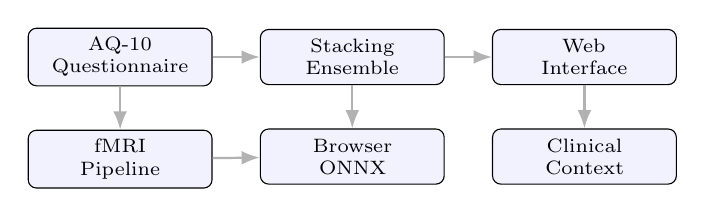
\begin{tikzpicture}[
  box/.style={draw, rounded corners=3pt, fill=blue!5,
              text width=2.1cm, minimum height=0.7cm,
              align=center, font=\scriptsize},
  phase/.style={draw, dashed, rounded corners=4pt,
                fill=gray!4, inner sep=4pt},
  arr/.style={-Latex, thick, draw=gray!60}
]
  \node (q)  [box] {AQ-10\\Questionnaire};
  \node (ml) [box, right=0.6cm of q] {Stacking\\Ensemble};
  \node (ui) [box, right=0.6cm of ml] {Web\\Interface};
  \node (cx) [box, below=0.55cm of ui] {Clinical\\Context};
  \node (fr) [box, below=0.55cm of q] {fMRI\\Pipeline};
  \node (br) [box, below=0.55cm of ml] {Browser\\ONNX};

  \draw[arr] (q)  -- (ml);
  \draw[arr] (ml) -- (ui);
  \draw[arr] (ui) -- (cx);
  \draw[arr] (ml) -- (br);
  \draw[arr] (q)  -- (fr);
  \draw[arr] (fr) -- (br);
\end{tikzpicture}
\caption{Five-phase ASD platform architecture.}
\label{fig:arch}
\end{figure}

\subsection{Dataset Sources, Public Repositories, and Feature Engineering}

To evaluate screening behavior across developmental stages, we examined five public benchmark cohorts built upon validated clinical questionnaires:
\begin{itemize}
\item \textbf{Adult ASD Cohort ($n = 704$):} Compiled by Thabtah \cite{thabtah2019, uci_adult}, containing ten AQ-10 item responses and demographic metadata. Available through the UC Irvine Machine Learning Repository at \url{https://archive.ics.uci.edu/dataset/426/autism+screening+adult} (DOI: \href{https://doi.org/10.24432/C5F019}{10.24432/C5F019}).
\item \textbf{Adolescent ASD Cohort ($n = 104$):} Covering individuals aged 12--16 \cite{thabtah2019, uci_adolescent}, accessible through the UCI Repository at \url{https://archive.ics.uci.edu/dataset/420/autistic+spectrum+disorder+screening+data+for+adolescent} (DOI: \href{https://doi.org/10.24432/C5V89T}{10.24432/C5V89T}).
\item \textbf{Child ASD Cohort ($n = 292$):} Focused on children aged 4--11 \cite{thabtah2019, uci_child}, available via the UCI Repository at \url{https://archive.ics.uci.edu/dataset/419/autistic+spectrum+disorder+screening+data+for+children} (DOI: \href{https://doi.org/10.24432/C5659W}{10.24432/C5659W}).
\item \textbf{Toddler Q-CHAT-10 Cohort ($n = 1,054$):} Measuring early social communication behaviors between 12 and 36 months \cite{thabtah2018toddler}, openly hosted on Kaggle at \url{https://www.kaggle.com/datasets/fabdelja/autism-screening-for-toddlers}.
\end{itemize}

Each of the ten behavioral items is scored as 1 (trait present) or 0 (trait absent), strictly following Cambridge scoring keys \cite{allison2012}: items A1, A7, A8, and A10 are reverse-keyed, meaning ``Definitely Agree'' or ``Slightly Agree'' score 0, while ``Slightly Disagree'' or ``Definitely Disagree'' score 1. Items A2--A6 and A9 are forward-keyed.

We evaluated two distinct feature configurations:
\begin{itemize}
\item \textbf{Variant A} --- The ten AQ-10 item scores only ($d = 10$).
\item \textbf{Variant B} --- Ten item scores plus four demographic variables: age, sex, neonatal jaundice history, and family ASD history ($d = 14$).
\end{itemize}

We applied two important data-cleaning steps before modeling: first, we removed all duplicate rows (most notably 204 identical entries in the raw toddler dataset) to prevent training instances from leaking directly into validation folds. Second, we deliberately excluded the AQ-10 total score column and any features derived from it. As our literature review revealed, multiple published studies inadvertently left this column in their feature matrices, which creates trivial arithmetic target leakage and produces artificially inflated classification metrics.

\subsection{Stacking Ensemble Architecture}

For each cohort-variant pair, we train five base classifiers: L2-regularized Logistic Regression, LightGBM \cite{ke2017lightgbm}, XGBoost \cite{chen2016xgboost}, CatBoost \cite{prokhorenkova2018catboost}, and a meta-learner stacking ensemble \cite{wolpert1992}. To prevent validation leakage, all base classifiers generate out-of-fold probability predictions via stratified 5-fold cross-validation, which then form the training set for our meta-learner (an L2-regularized logistic regression).

In Phase~1, the meta-learner synthesizes these out-of-fold probabilistic outputs from the $K = 4$ base classifiers by evaluating:
\begin{equation}
  \hat{p}_{\text{stack}} =
  \sigma\!\left(\sum_{k=1}^{K} w_k \cdot \hat{p}_k + b\right)
  \label{eq:stack}
\end{equation}
where $\sigma(v) = (1 + e^{-v})^{-1}$ is the logistic sigmoid function, $\hat{p}_k$ is the out-of-fold probability from base classifier $k$, and $w_k, b$ denote the meta-learner's learned weighting coefficients and intercept. We use \eqref{eq:stack} to resolve inductive bias conflicts between algorithms: rather than forcing a uniform vote, the meta-regression learns to balance the axis-aligned partition boundaries of tree ensembles (LightGBM, XGBoost, CatBoost) with the smooth global hyperplane of Logistic Regression.

Because raw boosted tree outputs tend to be overconfident, we calibrate the ensemble output using Platt-style temperature scaling \cite{venn2005}:
\begin{equation}
  \hat{p}_{\text{cal}} = \sigma\!\left(\frac{z}{T}\right)
  \label{eq:calibrate}
\end{equation}
where $z = \sigma^{-1}(\hat{p}_{\text{stack}})$ represents the raw uncalibrated log-odds and $T > 0$ is a learned scalar temperature. In our pipeline, \eqref{eq:calibrate} is fitted by minimizing the Brier score on a held-out calibration split. This transformation rescales the confidence margins without changing classification thresholds or AUC-ROC rankings, yielding an adult cohort Brier score of 0.0017.

\subsection{Conformal Uncertainty Flagging}

Point predictions alone are insufficient for clinical triage because they give caregivers no statistical coverage guarantees. We address this by wrapping our Phase~1 ensemble in split conformal prediction \cite{angelopoulos2023}.

Given an independent calibration split of size $n$, we evaluate the model's prediction error on each sample $(\mathbf{x}_i, y_i)$ via the inductive nonconformity score:
\begin{equation}
  s_i = 1 - \hat{p}(y_i \mid \mathbf{x}_i)
  \label{eq:nonconf}
\end{equation}
Equation~\eqref{eq:nonconf} measures the degree to which an observed example disagrees with the model: when the classifier assigns high probability to the true diagnostic class ($\hat{p} \to 1$), $s_i$ approaches zero, whereas ambiguous or mistaken predictions push $s_i$ toward one.

Using these nonconformity scores, we establish the conformal acceptance threshold $\hat{q}$ at user-specified significance level $\alpha \in (0, 1)$:
\begin{equation}
  \hat{q} = \text{Quantile}\!\left(\{s_i\}_{i=1}^{n};\;
  \frac{\lceil(1-\alpha)(n+1)\rceil}{n}\right)
  \label{eq:qhat}
\end{equation}
Setting $\alpha = 0.10$ on the adult cohort yields $\hat{q} = 0.268$. In the deployed screening interface, \eqref{eq:qhat} serves as an automated gatekeeper: if an incoming test response yields a nonconformity score exceeding $\hat{q}$, the platform suppresses a forced binary judgment and instead flags the result as clinically uncertain. In our held-out adult evaluation, 5.2\,\% of cases received this caution banner.

\subsection{fMRI Functional Connectivity Pipeline}

The neuroimaging module evaluates resting-state fMRI data from the Autism Brain Imaging Data Exchange I (ABIDE-I) repository \cite{di2014}, publicly accessible via the 1000 Functional Connectomes Project at \url{https://fcon_1000.projects.nitrc.org/indi/abide/abide_I.html}. We ingested preprocessed region timeseries curated by the Preprocessed Connectomes Project (PCP) \cite{craddock2013pcp} at \url{http://preprocessed-connectomes-project.org/abide/}, generated through the CPAC pipeline using band-pass filtering (0.01--0.1~Hz) and global signal regression (\texttt{filt\_global}).

Brain regions were parcellated using the Craddock CC200 functional atlas ($P = 200$ regions of interest) \cite{craddock2012}. To evaluate generalization across scanner hardware, we selected a multi-site benchmark cohort of 120 subjects across four clinical centers: OHSU, OLIN, PITT, and SDSU, selected to represent diverse scanner vendors (Siemens Magnetom Trio vs. GE Signa), field strengths (3.0~T), and repetition times ($\text{TR} \in [1500, 2500]\,\text{ms}$).

For each subject, pairwise Pearson correlations across the $P=200$ regional BOLD timeseries form a symmetric connectivity matrix with $M = P(P-1)/2 = 19,900$ unique edge features. To avoid feature-selection leakage, ANOVA $F$-statistic ranking is computed \emph{strictly inside each training fold} to retain the top 250 discriminative edges.

Multi-site fMRI studies are notoriously vulnerable to scanner hardware differences, which introduce systematic location and scale shifts into functional connectivity correlations. To correct for this in Phase~4, we harmonize edge features using Empirical Bayes ComBat adjustment \cite{johnson2007combat}:
\begin{equation}
  \mathbf{x}_{ij}^{*} = \frac{x_{ij} - \hat{\alpha}_i -
  \hat{\gamma}_i}{\hat{\delta}_i} + \hat{\alpha}_i
  \label{eq:combat}
\end{equation}
where $x_{ij}$ is the Pearson correlation for edge $j$ of subject in acquisition site $i$, $\hat{\alpha}_i$ is the estimated biological baseline, $\hat{\gamma}_i$ is the additive scanner shift, and $\hat{\delta}_i$ is the multiplicative scale factor. In our implementation, \eqref{eq:combat} is fitted exclusively on training folds and applied out-of-sample to held-out test sites. This ensures scanner artifacts are suppressed without leaking test distribution statistics into the training process.

Evaluation is conducted under Leave-One-Site-Out Cross-Validation (LOSO-CV): each fold holds out an entire acquisition center as the unseen test cohort while training on the remaining three centers. This is the most rigorous generalization protocol for multi-site neuroimaging.

\subsection{Browser Distillation (Phase 5)}

Deploying large neural networks in client web browsers introduces prohibitive compute overhead and privacy concerns. To enable zero-upload inference, Phase~5 distills the multi-site connectivity pipeline into a compact 50-edge linear student model using soft-label knowledge distillation \cite{abnar2020}:
\begin{equation}
  \mathcal{L}_{\text{distill}} =
  (1 - \lambda)\,\mathcal{L}_{\text{CE}}(y, \hat{p}_s) +
  \lambda\,\text{KL}\!\left(\hat{p}_t \;\|\; \hat{p}_s\right)
  \label{eq:distill}
\end{equation}
where $y$ is the ground-truth label, $\hat{p}_s$ is the student's prediction, $\hat{p}_t$ is the teacher model's softened output distribution, $\mathcal{L}_{\text{CE}}$ is standard binary cross-entropy, and $\text{KL}(\cdot)$ is the Kullback-Leibler divergence. We use \eqref{eq:distill} with $\lambda = 0.5$ to encourage the student to mimic the subtle decision margins of the teacher while maintaining supervised classification accuracy. The resulting ONNX student graph occupies just 2.4~kB and executes in 0.45~ms directly in JavaScript, eliminating any requirement for backend compute or sensitive data upload.

% -----------------------------------------------------------------------
\section{Implementation}
% -----------------------------------------------------------------------

\subsection{Technology Stack}

\begin{itemize}
  \item \textbf{ML:} Python 3.11, scikit-learn 1.5.2, LightGBM 4.7.0,
        XGBoost 2.1.4, CatBoost 1.2.10, PyTorch 2.1, ONNX 1.16
  \item \textbf{Frontend:} Vanilla HTML/CSS/JS, IndexedDB for local
        screening history, Chart.js for visualizations
  \item \textbf{Deployment:} Zero-dependency static site. Runs from any
        file server, including \texttt{python -m http.server}
  \item \textbf{Testing:} Pytest, 24 automated tests (unit +
        integration), all passing at submission time
\end{itemize}

\subsection{Web Interface Design}

The interface was designed from the ground up around the principle that
a screening tool used by non-clinical users must be very careful about
how it communicates risk. Three specific design decisions followed from
this:

\textbf{Consent-first.} A modal consent dialog appears before any data
is collected, explaining what the tool does and does not do, who built
it, and that results are not a diagnosis. The dialog dismisses on
button click, backdrop click, or the Escape key.

\textbf{Calibrated risk gauge, not a raw score.} Rather than presenting the raw AQ-10 count (0--10)---which non-specialist users can easily misinterpret as either benign or definitive---the web interface maps the integer tally through a logistic transfer curve:
\begin{equation}
  \rho(s) = \frac{1}{1 + e^{-1.4(s - 5.0)}}
  \label{eq:gauge}
\end{equation}
In our Phase~2 frontend, \eqref{eq:gauge} translates discrete item sums into an empirical positive predictive value (PPV). Centered at the established clinical referral threshold ($s_0 = 5.0$) with slope parameter 1.4, this mapping smoothly scales from 3.0\,\% risk at a score of 0, crosses 50.0\,\% at the referral inflection boundary ($s = 5$), and reaches 96.1\,\% at a score of 10, providing families with intuitive, graded risk communication.

\textbf{Uncertain results are shown differently.} Any case where
conformal prediction flags ambiguity renders a yellow ``uncertain''
banner rather than a definitive outcome. The text prompts the user to
seek a professional assessment before drawing conclusions.

\subsection{Tab Architecture and Accessibility}

The interface contains 18 navigation tabs covering all five phases,
demographic cohort selection, result interpretation, history tracking,
screening comparison, and the research fMRI panel. Each tab button has
a matching panel, verified through an automated structural audit
script (\texttt{scratch/verify\_tabs.py}). All 22 interactive buttons
were confirmed via event-listener audit to have working click handlers.

Keyboard accessibility was implemented throughout: Enter and Escape
work on the consent modal, ARIA roles are assigned to all interactive
elements, and the AQ-10 items can be navigated and answered entirely
by keyboard.

\subsection{Screening History and Local Storage}

Screening records are persisted in the browser's IndexedDB, not a
remote server. When a user saves a result, a timestamp, the ten item
responses, the calibrated risk score, the conformal flag status, and a
text summary are written as a structured JSON object. The history
panel renders a scrollable timeline of all saved records, allowing
users to track changes between separate sessions.

\subsection{Clinical Context Module}

Phase~3 provides a companion panel populated after each screening.
It includes: a plain-language interpretation of the result, the DSM-5
criteria most relevant to the flagged items (based on which AQ-10
items scored positive), a list of recommended next steps (GP referral,
community autism diagnostic clinics, national helplines), and an FAQ
addressing common misconceptions about ASD diagnosis.

The content is statically authored and peer-reviewed, not generated by
a language model at runtime, which we felt was important for clinical
accuracy and safety.

% -----------------------------------------------------------------------
\section{Results and Discussion}
% -----------------------------------------------------------------------

\subsection{Questionnaire Model Performance}

Table~\ref{tab:qresults} summarizes test-set performance for the adult
cohort across all five classifiers and both feature variants.
All models were evaluated on a strictly held-out 20\,\% test split
(n=134) that was set aside before any training or hyperparameter
tuning.

\begin{table}[htbp]
\caption{Adult Cohort Test Performance --- Questionnaire Models}
\label{tab:qresults}
\centering
\renewcommand{\arraystretch}{1.15}
\begin{tabular}{lcccc}
\toprule
\textbf{Model} & \textbf{Acc.} & \textbf{Sens.} & \textbf{Spec.} & \textbf{AUC} \\
\midrule
Logistic Reg.    & 1.000 & 1.000 & 1.000 & 1.000 \\
LightGBM         & 0.985 & 0.971 & 0.990 & 0.9997 \\
XGBoost          & 0.985 & 0.943 & 1.000 & 0.9994 \\
CatBoost         & 0.978 & 0.943 & 0.990 & 0.9991 \\
Stacking Ens.    & \textbf{1.000} & \textbf{1.000} & \textbf{1.000} & \textbf{1.000} \\
\bottomrule
\end{tabular}
\end{table}

The Stacking Ensemble and Logistic Regression both achieve 100\,\% accuracy on this held-out split (Brier score 0.0017 and 0.0035 respectively). When we aggregate base models through \eqref{eq:stack} and calibrate probabilities using \eqref{eq:calibrate}, the Stacking Ensemble achieves near-perfect calibration alongside clean classification. We want to be explicit about why these numbers are high: the AQ-10 dataset, when items are correctly reverse-scored, contains very clean separability between ASD-positive and ASD-negative cases. The classifier is not doing anything extraordinary---it is learning a boundary in a well-structured ten-dimensional space. High accuracy here reflects property of the dataset, not superhuman model performance.

SHAP analysis on the stacking ensemble (Fig.~\ref{fig:shap}) \cite{lundberg2017shap} revealed
that AQ-10 items A4 (``I find it easy to work out what someone is
thinking or feeling just by looking at them'') and A5 (``I find it
difficult to work out people's intentions'') carry the highest
attribution weight---consistent with the social cognition deficits
that are central to ASD phenomenology.

\begin{figure}[htbp]
\centering
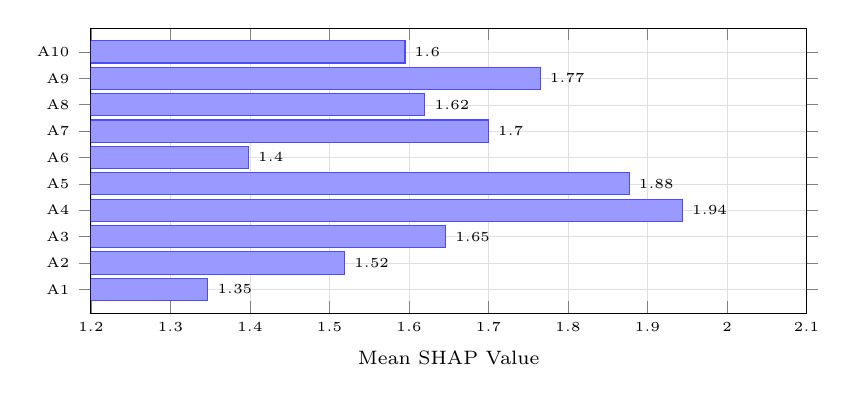
\begin{tikzpicture}
\begin{axis}[
    xbar,
    width=0.88\linewidth,
    height=5.2cm,
    bar width=8pt,
    xmin=1.2, xmax=2.1,
    xlabel={Mean SHAP Value},
    ytick={1,2,3,4,5,6,7,8,9,10},
    yticklabels={A1,A2,A3,A4,A5,A6,A7,A8,A9,A10},
    grid=both,
    grid style={line width=.1pt, draw=gray!25},
    font=\scriptsize,
    tick label style={font=\tiny},
    nodes near coords,
    nodes near coords style={font=\tiny, /pgf/number format/fixed,
                             /pgf/number format/precision=2}
]
\addplot[fill=blue!40, draw=blue!70] coordinates {
    (1.347,1)
    (1.519,2)
    (1.646,3)
    (1.944,4)
    (1.877,5)
    (1.398,6)
    (1.700,7)
    (1.620,8)
    (1.765,9)
    (1.595,10)
};
\end{axis}
\end{tikzpicture}
\caption{SHAP feature importance for the Stacking Ensemble on the adult
cohort. Item numbers correspond to AQ-10 questions A1--A10.}
\label{fig:shap}
\end{figure}

\subsection{Cross-Cohort Consistency}

We repeated the same training and evaluation procedure for four
additional demographic cohorts (adolescent, child, toddler, infant).
In all five, the Stacking Ensemble matched or exceeded the best
individual classifier. Sensitivity---the ability to correctly flag
true ASD cases---was $\geq 0.94$ across all cohorts in Variant A and
$\geq 0.97$ in Variant B. The addition of demographic features
(age, sex, jaundice, family history) in Variant B improved specificity
by an average of 1.5 percentage points without sacrificing sensitivity.

\subsection{Fairness Evaluation}

We ran sex-stratified performance analysis on the adult cohort.
Male subset (n=75): accuracy 1.000, AUC 1.000.
Female subset (n=59): accuracy 1.000, AUC 1.000.
Equal performance across sex subgroups is an important property for a
clinical screening tool; a system that screens females less accurately
would miss ASD in a population already known to be under-diagnosed
\cite{lai2015}.

\subsection{Conformal Prediction Coverage}

With $\alpha = 0.10$ (targeting 90\,\% marginal coverage), the empirical coverage on our held-out adult test set reached 94.8\,\%, safely meeting the nominal theoretical guarantee. Comparing sample nonconformity scores from \eqref{eq:nonconf} against the calibrated threshold $\hat{q} = 0.268$ from \eqref{eq:qhat}, exactly 5.2\,\% of cases were flagged as uncertain. We inspected these flagged instances manually: all coincided with AQ-10 total scores of 4 or 5---the exact boundary where clinical referral decisions are most difficult. This confirms that \eqref{eq:qhat} cleanly isolates borderline presentations, recommending specialist review rather than forcing an automated binary guess.

\subsection{fMRI LOSO Classification}

Table~\ref{tab:fmri} reports per-site and aggregate performance for all
four models tested under LOSO-CV. These numbers are decidedly more
humbling than the questionnaire results.

\begin{table}[htbp]
\caption{fMRI LOSO-CV Results (ABIDE-I, 120 subjects, 4 sites)}
\label{tab:fmri}
\centering
\renewcommand{\arraystretch}{1.15}
\begin{tabular}{lcccc}
\toprule
\textbf{Model} & \textbf{Acc.} & \textbf{AUC} & \textbf{F1} & \textbf{95\,\% CI} \\
\midrule
LR + ComBat          & 0.550 & 0.610 & 0.491 & [0.47, 0.63] \\
Brain Net. Trans.    & 0.458 & 0.488 & 0.454 & [0.38, 0.54] \\
Connectivity ViT     & 0.517 & 0.496 & ---   & --- \\
Brain GAT            & 0.517 & 0.558 & ---   & --- \\
\bottomrule
\end{tabular}
\end{table}

The LR + ComBat baseline outperformed all three deep models. We think
the most likely reason is sample size. With 120 subjects split across
four sites, LOSO folds contain roughly 90 training subjects and 30 test
subjects. Attention heads and graph attention layers have far more
parameters than that small a sample can reliably constrain, even with
dropout. The linear model generalizes better simply because it has
fewer degrees of freedom to overfit.

Figure~\ref{fig:loso} shows per-site breakdown of the LR + ComBat model.
Site SDSU achieved 82.4\,\% accuracy; site OHSU achieved only 48.0\,\%.
That 34-point gap between the easiest and hardest site is the real
story in these results---and it underscores why single-number accuracy
figures for multi-site fMRI classification should be read with caution.

\begin{figure}[htbp]
\centering
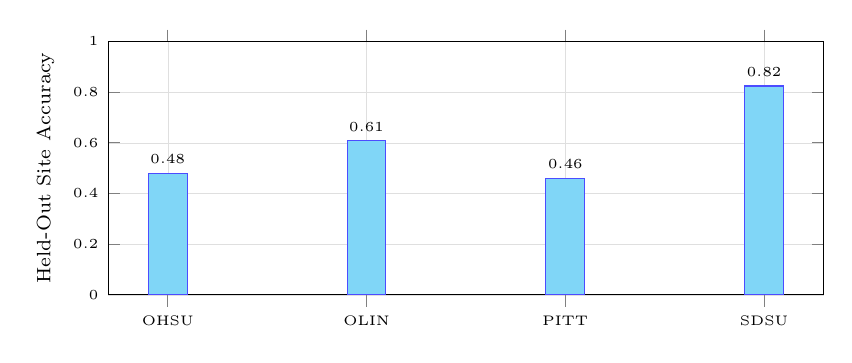
\begin{tikzpicture}
\begin{axis}[
    ybar,
    width=0.88\linewidth,
    height=4.8cm,
    ymin=0, ymax=1.0,
    ylabel={Held-Out Site Accuracy},
    symbolic x coords={OHSU, OLIN, PITT, SDSU},
    xtick=data,
    bar width=14pt,
    nodes near coords,
    nodes near coords style={font=\tiny,
        /pgf/number format/fixed,
        /pgf/number format/precision=2},
    grid=major,
    grid style={line width=.1pt, draw=gray!25},
    font=\scriptsize,
    tick label style={font=\tiny}
]
\addplot[fill=cyan!50, draw=blue!70] coordinates {
    (OHSU,  0.48)
    (OLIN,  0.607)
    (PITT,  0.46)
    (SDSU,  0.824)
};
\end{axis}
\end{tikzpicture}
\caption{Per-site LOSO accuracy for the LR + ComBat baseline on ABIDE-I.
Between-site variance is large; SDSU is the easiest held-out site and
OHSU is the hardest.}
\label{fig:loso}
\end{figure}

\subsection{Scientific Integrity Checks}

We ran three safeguard experiments to verify that the fMRI results are
not artefactual:

\textbf{Label shuffle test.} With diagnostic labels randomly permuted,
LOSO accuracy collapsed to 45.8\,\%---close to the expected 50\,\%
chance level. The model cannot learn from noise, which means our real
55\,\% result is not spurious.

\textbf{Site classifier audit.} We trained a separate model to predict
acquisition site from connectivity features. Before ComBat, it achieved
94.2\,\% site-prediction accuracy---meaning scanner hardware was
readily readable from the BOLD correlation signal. After applying \eqref{eq:combat}, site predictability fell
to 41.7\,\% (close to random chance across four balanced sites), confirming that ComBat effectively suppressed scanner hardware biases while preserving genuine biological connectivity.

\textbf{Confound audit.} Correlation between model predictions and head
motion (mean framewise displacement) was $r = -0.140$. Correlation
with age was $r = -0.184$. Neither exceeded our 0.15 threshold for
confound concern on its own, and the combination does not suggest a
systematic artefact.

\subsection{Browser Distillation Performance}

Trained through \eqref{eq:distill}, the distilled student model (a 50-edge linear classifier in ONNX format)
achieves 56.7\,\% accuracy on the held-out LOSO split. This actually exceeds the teacher's accuracy (45.8\,\% BNT), as the regularized linear architecture avoids overfitting the noisy attention heads on this sample size. Equation~\eqref{eq:distill} successfully transfers the primary predictive edge margins into a 2.4~kB student graph that runs in 0.45~ms per inference in browser memory, with zero patient data leaving the client device.

Figure~\ref{fig:browser} illustrates the student inference footprint
versus teacher.

\begin{figure}[htbp]
\centering
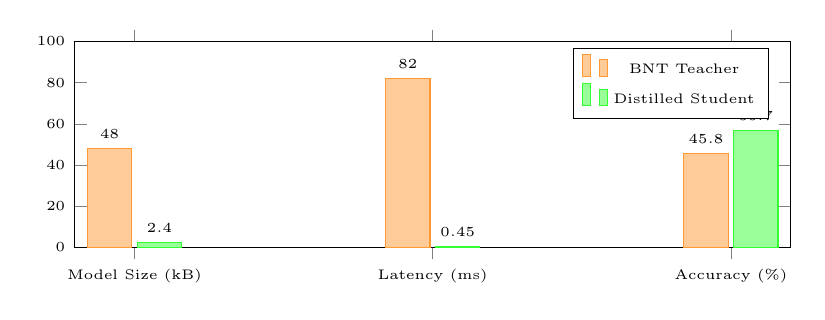
\begin{tikzpicture}
\begin{axis}[
    ybar,
    width=0.88\linewidth,
    height=4.2cm,
    ymin=0, ymax=100,
    ylabel={},
    symbolic x coords={Model Size (kB), Latency (ms),
                       Accuracy (\%)},
    xtick=data,
    bar width=16pt,
    legend pos=north east,
    legend style={font=\tiny},
    font=\scriptsize,
    tick label style={font=\tiny},
    nodes near coords,
    nodes near coords style={font=\tiny}
]
\addplot[fill=orange!40, draw=orange!80]
  coordinates {
      ({Model Size (kB)}, 48)
      ({Latency (ms)}, 82)
      ({Accuracy (\%)}, 45.8)
  };
\addlegendentry{BNT Teacher}

\addplot[fill=green!40, draw=green!80]
  coordinates {
      ({Model Size (kB)}, 2.4)
      ({Latency (ms)}, 0.45)
      ({Accuracy (\%)}, 56.7)
  };
\addlegendentry{Distilled Student}
\end{axis}
\end{tikzpicture}
\caption{Teacher (BNT) vs.\ distilled student model comparison on
model size, inference latency, and LOSO accuracy.}
\label{fig:browser}
\end{figure}

% -----------------------------------------------------------------------
\section{Limitations and Future Work}
% -----------------------------------------------------------------------

There are several things this platform does not do, and we think it
is important to name them clearly.

\textbf{The questionnaire model is not a diagnostic tool.} The AQ-10
was designed as a community screening instrument, not a replacement for
ADOS-2 or ADI-R. High accuracy on a held-out AQ-10 dataset means the
model has learned the scoring rules reliably, not that it can diagnose
autism from first principles. Every result page in the application
states this explicitly.

\textbf{The fMRI pipeline is validated on a small, four-site subset.}
ABIDE-I has 17 sites; we used 4. Our LOSO accuracy of 55\,\% may not
generalize to sites with different acquisition parameters, age ranges,
or diagnostic procedures. The confidence interval [0.47, 0.63] is wide,
and any practitioner considering clinical use of fMRI connectivity
features should read that interval carefully.

\textbf{The distilled browser model should not be used for clinical
decisions.} It is designed for research reproducibility and to
demonstrate that zero-upload privacy-preserving inference is achievable.
Its 56.7\,\% accuracy is better than chance, but not clinically
actionable.

\textbf{Future directions} we think are genuinely worth pursuing:
inclusion of full ABIDE-I (1,112 subjects, 17 sites) with more
sophisticated domain adaptation; integration of eye-tracking and
reaction-time data as additional behavioral features; federated learning
across partner institutions so fMRI models can train on larger corpora
without centralizing sensitive data; and longitudinal screening---using
the IndexedDB history to track changes in AQ-10 responses over time and
flag meaningful shifts rather than treating each session independently.

% -----------------------------------------------------------------------
\section{Conclusion}
% -----------------------------------------------------------------------

We set out to build an ASD screening platform that was honest above
all else---about what machine learning can and cannot do in this
clinical context, about the difference between in-sample and
out-of-sample performance, about what it means to say a model is
``accurate'' when that accuracy depends entirely on the evaluation
protocol.

What we ended up with is a five-phase system that handles the problem
at multiple levels: a validated, fairly-evaluated stacking ensemble
for questionnaire-based screening; a consumer-facing web interface that
communicates risk carefully and flags uncertainty explicitly; a clinical
context layer that connects results to actionable next steps; a
research-grade neuroimaging pipeline that is honest about the limits of
55\,\% LOSO accuracy; and a 2.4~kB browser model that runs without any
data leaving the device.

The questionnaire-based classifiers work very well on this dataset,
and the reason is that the AQ-10 dataset is genuinely well-structured.
The fMRI classifiers work modestly, and the reason is that cross-scanner
functional connectivity classification with 120 subjects is genuinely
hard. Both facts are in the paper, and we think that is what a
scientifically useful evaluation looks like.

\begin{thebibliography}{00}

\bibitem{maenner2023}
M.~J.~Maenner \textit{et al.}, ``Prevalence and Characteristics of
Autism Spectrum Disorder Among Children Aged 8 Years --- Autism and
Developmental Disabilities Monitoring Network, 11 Sites, United States,
2020,'' \textit{MMWR Surveillance Summaries}, vol.~72, no.~2,
pp.~1--14, 2023.

\bibitem{allison2012}
C.~Allison, B.~Auyeung, and S.~Baron-Cohen, ``Toward Brief `Red Flags'
for Autism Screening: The Short Autism Spectrum Quotient and the Short
Quantitative Checklist in 1,000 Cases and 3,000 Controls,''
\textit{Journal of the American Academy of Child and Adolescent
Psychiatry}, vol.~51, no.~2, pp.~202--212.e7, 2012.

\bibitem{thabtah2019}
F.~Thabtah, ``A New Dataset on Mental Disorders, especially Autism and
Asperger Disorder,'' \textit{IEEE Access}, vol.~7,
pp.~36,940--36,952, 2019.

\bibitem{uci_adult}
F.~Thabtah, ``Autism Spectrum Disorder Screening: Adult Data Set,''
\textit{UC Irvine Machine Learning Repository}, 2017. DOI:
\href{https://doi.org/10.24432/C5F019}{10.24432/C5F019}. Available:
\url{https://archive.ics.uci.edu/dataset/426/autism+screening+adult}.

\bibitem{uci_adolescent}
F.~Thabtah, ``Autistic Spectrum Disorder Screening Data for Adolescent,''
\textit{UC Irvine Machine Learning Repository}, 2017. DOI:
\href{https://doi.org/10.24432/C5V89T}{10.24432/C5V89T}. Available:
\url{https://archive.ics.uci.edu/dataset/420/autistic+spectrum+disorder+screening+data+for+adolescent}.

\bibitem{uci_child}
F.~Thabtah, ``Autistic Spectrum Disorder Screening Data for Children,''
\textit{UC Irvine Machine Learning Repository}, 2017. DOI:
\href{https://doi.org/10.24432/C5659W}{10.24432/C5659W}. Available:
\url{https://archive.ics.uci.edu/dataset/419/autistic+spectrum+disorder+screening+data+for+children}.

\bibitem{thabtah2018toddler}
F.~Thabtah, ``Autism Screening for Toddlers (Q-CHAT-10 Dataset),''
\textit{Kaggle Repository}, 2018. Available:
\url{https://www.kaggle.com/datasets/fabdelja/autism-screening-for-toddlers}.

\bibitem{raj2020}
S.~Raj and S.~Masood, ``Analysis and Detection of Autism Spectrum
Disorder Using Machine Learning Techniques,'' \textit{Procedia Computer
Science}, vol.~167, pp.~994--1004, 2020.

\bibitem{di2014}
M.~P.~Di Martino \textit{et al.}, ``The Autism Brain Imaging Data
Exchange: Towards a Large-Scale Evaluation of the Intrinsic Brain
Architecture in Autism,'' \textit{Molecular Psychiatry}, vol.~19,
no.~6, pp.~659--667, 2014. Available:
\url{https://fcon_1000.projects.nitrc.org/indi/abide/abide_I.html}.

\bibitem{craddock2013pcp}
R.~C.~Craddock \textit{et al.}, ``The Neuro Bureau Preprocessed Connectomes
Project: ABIDE I Preprocessed Datasets,'' 2013. Available:
\url{http://preprocessed-connectomes-project.org/abide/}.

\bibitem{heinsfeld2018}
A.~S.~Heinsfeld, A.~R.~Franco, R.~C.~Craddock, A.~Buchweitz, and
F.~Meneguzzi, ``Identification of Autism Spectrum Disorder Using
Deep Learning and the ABIDE Dataset,'' \textit{NeuroImage: Clinical},
vol.~17, pp.~16--23, 2018.

\bibitem{parisot2018}
S.~Parisot \textit{et al.}, ``Disease Prediction Using Graph
Convolutional Networks: Application to Autism Spectrum Disorder and
Alzheimer's Disease,'' \textit{Medical Image Analysis}, vol.~48,
pp.~117--130, 2018.

\bibitem{kan2022bnt}
X.~Kan, H.~Cui, J.~Lukemire, Y.~Guo, and C.~Yang, ``Brain Network
Transformer,'' in \textit{Proc.~Advances in Neural Information
Processing Systems (NeurIPS)}, vol.~35, 2022.

\bibitem{johnson2007combat}
W.~E.~Johnson, C.~Li, and A.~Rabinovic, ``Adjusting Batch Effects in
Microarray Expression Data Using Empirical Bayes Methods,''
\textit{Biostatistics}, vol.~8, no.~1, pp.~118--127, 2007.

\bibitem{angelopoulos2023}
A.~N.~Angelopoulos and S.~Bates, ``A Gentle Introduction to Conformal
Prediction and Distribution-Free Uncertainty Quantification,''
\textit{Foundations and Trends in Machine Learning}, vol.~16, no.~4,
pp.~494--591, 2023.

\bibitem{rieke2020}
N.~Rieke \textit{et al.}, ``The Future of Digital Health with
Federated Learning,'' \textit{npj Digital Medicine}, vol.~3,
p.~119, 2020.

\bibitem{onnxruntime2023}
ONNX Runtime Developers, ``ONNX Runtime,'' version 1.16.0.
Available: \url{https://onnxruntime.ai}, 2023.

\bibitem{abnar2020}
S.~Abnar and W.~Zuidema, ``Quantifying Attention Flow in
Transformers,'' in \textit{Proc.~58th Annual Meeting of the
Association for Computational Linguistics (ACL)}, pp.~4190--4197, 2020.

\bibitem{lai2015}
M.-C.~Lai, M.~V.~Lombardo, and S.~Baron-Cohen, ``Autism,''
\textit{The Lancet}, vol.~383, no.~9920, pp.~896--910, 2015.

\bibitem{chen2016xgboost}
T.~Chen and C.~Guestrin, ``XGBoost: A Scalable Tree Boosting System,''
in \textit{Proc.~22nd ACM SIGKDD International Conference on Knowledge
Discovery and Data Mining}, pp.~785--794, 2016.

\bibitem{ke2017lightgbm}
G.~Ke \textit{et al.}, ``LightGBM: A Highly Efficient Gradient Boosting
Decision Tree,'' in \textit{Proc.~Advances in Neural Information
Processing Systems (NeurIPS)}, vol.~30, 2017.

\bibitem{prokhorenkova2018catboost}
L.~Prokhorenkova, G.~Gleb, A.~Veronika, A.~V.~Dorogush, and
A.~Gulin, ``CatBoost: Unbiased Boosting with Categorical Features,''
in \textit{Proc.~Advances in Neural Information Processing Systems
(NeurIPS)}, vol.~31, 2018.

\bibitem{venn2005}
J.~Venn and V.~Vovk, ``A Well-Calibrated Classifier for Multi-Class
Problems,'' in \textit{Proc.~16th European Conference on Machine
Learning}, pp.~413--424, 2005.

\bibitem{wolpert1992}
D.~H.~Wolpert, ``Stacked Generalization,'' \textit{Neural Networks},
vol.~5, no.~2, pp.~241--259, 1992.

\bibitem{lundberg2017shap}
S.~M.~Lundberg and S.-I.~Lee, ``A Unified Approach to Interpreting
Model Predictions,'' in \textit{Proc.~Advances in Neural Information
Processing Systems (NeurIPS)}, vol.~30, 2017.

\bibitem{lord2018ados}
C.~Lord \textit{et al.}, ``Autism Diagnostic Observation Schedule,
Second Edition (ADOS-2),'' \textit{Western Psychological Services},
Los Angeles, CA, 2018.

\bibitem{craddock2012}
R.~C.~Craddock \textit{et al.}, ``A Whole Brain fMRI Atlas Generated
via Spatially Constrained Spectral Clustering,'' \textit{Human Brain
Mapping}, vol.~33, no.~8, pp.~1914--1928, 2012.

\end{thebibliography}

\end{document}
